% Options for packages loaded elsewhere
\PassOptionsToPackage{unicode}{hyperref}
\PassOptionsToPackage{hyphens}{url}
%
\documentclass[
]{book}
\usepackage{amsmath,amssymb}
\usepackage{lmodern}
\usepackage{ifxetex,ifluatex}
\ifnum 0\ifxetex 1\fi\ifluatex 1\fi=0 % if pdftex
  \usepackage[T1]{fontenc}
  \usepackage[utf8]{inputenc}
  \usepackage{textcomp} % provide euro and other symbols
\else % if luatex or xetex
  \usepackage{unicode-math}
  \defaultfontfeatures{Scale=MatchLowercase}
  \defaultfontfeatures[\rmfamily]{Ligatures=TeX,Scale=1}
\fi
% Use upquote if available, for straight quotes in verbatim environments
\IfFileExists{upquote.sty}{\usepackage{upquote}}{}
\IfFileExists{microtype.sty}{% use microtype if available
  \usepackage[]{microtype}
  \UseMicrotypeSet[protrusion]{basicmath} % disable protrusion for tt fonts
}{}
\makeatletter
\@ifundefined{KOMAClassName}{% if non-KOMA class
  \IfFileExists{parskip.sty}{%
    \usepackage{parskip}
  }{% else
    \setlength{\parindent}{0pt}
    \setlength{\parskip}{6pt plus 2pt minus 1pt}}
}{% if KOMA class
  \KOMAoptions{parskip=half}}
\makeatother
\usepackage{xcolor}
\IfFileExists{xurl.sty}{\usepackage{xurl}}{} % add URL line breaks if available
\IfFileExists{bookmark.sty}{\usepackage{bookmark}}{\usepackage{hyperref}}
\hypersetup{
  pdftitle={Vacunación COVID-19 en Docentes},
  pdfauthor={Bio-Math Team},
  hidelinks,
  pdfcreator={LaTeX via pandoc}}
\urlstyle{same} % disable monospaced font for URLs
\usepackage{longtable,booktabs,array}
\usepackage{calc} % for calculating minipage widths
% Correct order of tables after \paragraph or \subparagraph
\usepackage{etoolbox}
\makeatletter
\patchcmd\longtable{\par}{\if@noskipsec\mbox{}\fi\par}{}{}
\makeatother
% Allow footnotes in longtable head/foot
\IfFileExists{footnotehyper.sty}{\usepackage{footnotehyper}}{\usepackage{footnote}}
\makesavenoteenv{longtable}
\usepackage{graphicx}
\makeatletter
\def\maxwidth{\ifdim\Gin@nat@width>\linewidth\linewidth\else\Gin@nat@width\fi}
\def\maxheight{\ifdim\Gin@nat@height>\textheight\textheight\else\Gin@nat@height\fi}
\makeatother
% Scale images if necessary, so that they will not overflow the page
% margins by default, and it is still possible to overwrite the defaults
% using explicit options in \includegraphics[width, height, ...]{}
\setkeys{Gin}{width=\maxwidth,height=\maxheight,keepaspectratio}
% Set default figure placement to htbp
\makeatletter
\def\fps@figure{htbp}
\makeatother
\setlength{\emergencystretch}{3em} % prevent overfull lines
\providecommand{\tightlist}{%
  \setlength{\itemsep}{0pt}\setlength{\parskip}{0pt}}
\setcounter{secnumdepth}{5}
\usepackage{booktabs}
\usepackage{amsthm}
\makeatletter
\def\thm@space@setup{%
  \thm@preskip=8pt plus 2pt minus 4pt
  \thm@postskip=\thm@preskip
}
\makeatother
\usepackage{booktabs}
\usepackage{longtable}
\usepackage{array}
\usepackage{multirow}
\usepackage{wrapfig}
\usepackage{float}
\usepackage{colortbl}
\usepackage{pdflscape}
\usepackage{tabu}
\usepackage{threeparttable}
\usepackage{threeparttablex}
\usepackage[normalem]{ulem}
\usepackage{makecell}
\usepackage{xcolor}
\ifluatex
  \usepackage{selnolig}  % disable illegal ligatures
\fi
\usepackage[]{natbib}
\bibliographystyle{apalike}

\title{Vacunación COVID-19 en Docentes}
\usepackage{etoolbox}
\makeatletter
\providecommand{\subtitle}[1]{% add subtitle to \maketitle
  \apptocmd{\@title}{\par {\large #1 \par}}{}{}
}
\makeatother
\subtitle{Exploración de Base de Datos}
\author{Bio-Math Team}
\date{2021-04-29}

\begin{document}
\maketitle

{
\setcounter{tocdepth}{1}
\tableofcontents
}
\hypertarget{descripciuxf3n-general-del-proyecto}{%
\chapter{Descripción General del Proyecto}\label{descripciuxf3n-general-del-proyecto}}

\hypertarget{EDA}{%
\chapter{Análisis Exploratorio de los Datos}\label{EDA}}

La base de datos \texttt{fullclass.csv} contiene las siguientes variables extras a \texttt{class.csv}:

\begin{itemize}
\tightlist
\item
  \emph{Teacher}
\end{itemize}

Se agregan las variables \texttt{FOBAP} y \texttt{RES}.

\hypertarget{diagnuxf3stico-general}{%
\section{Diagnóstico General}\label{diagnuxf3stico-general}}

\begin{table}[H]
\centering
\begin{tabular}[t]{l|l|r|r|r|r}
\hline
variables & types & missing\_count & missing\_percent & unique\_count & unique\_rate\\
\hline
genero & factor & 3 & 1.345292 & 4 & 0.0179372\\
\hline
edad & ordered & 5 & 2.242152 & 6 & 0.0269058\\
\hline
grado\_academico & ordered & 3 & 1.345292 & 4 & 0.0179372\\
\hline
estado\_residencia & factor & 11 & 4.932735 & 16 & 0.0717489\\
\hline
habitantes\_en\_casa & ordered & 50 & 22.421525 & 5 & 0.0224215\\
\hline
enfermedades & character & 9 & 4.035874 & 21 & 0.0941704\\
\hline
nivel\_educativo\_clases & character & 14 & 6.278027 & 23 & 0.1031390\\
\hline
modalidad\_clases & factor & 5 & 2.242152 & 6 & 0.0269058\\
\hline
horas\_trabajo\_onsite & character & 137 & 61.434978 & 6 & 0.0269058\\
\hline
horas\_trabajo\_diarias & ordered & 28 & 12.556054 & 5 & 0.0224215\\
\hline
Danger & numeric & 0 & 0.000000 & 24 & 0.1076233\\
\hline
Xeno & numeric & 0 & 0.000000 & 25 & 0.1121076\\
\hline
Socio & numeric & 0 & 0.000000 & 35 & 0.1569507\\
\hline
Con & numeric & 0 & 0.000000 & 24 & 0.1076233\\
\hline
Trauma & numeric & 0 & 0.000000 & 24 & 0.1076233\\
\hline
Comp & numeric & 0 & 0.000000 & 24 & 0.1076233\\
\hline
Level & ordered & 0 & 0.000000 & 4 & 0.0179372\\
\hline
FOBAP & integer & 0 & 0.000000 & 9 & 0.0403587\\
\hline
RES & integer & 0 & 0.000000 & 18 & 0.0807175\\
\hline
\end{tabular}
\end{table}

\textbf{Dudas:}

\begin{itemize}
\tightlist
\item
  ¿Las variables están en las escalas de medición correcta para cada uno?
\item
  Si no es así, ¿cuáles debemos cambiar y a qué tipo de escala?
\end{itemize}

\hypertarget{anuxe1lisis-univariado}{%
\section{Análisis Univariado}\label{anuxe1lisis-univariado}}

\begin{verbatim}
## data 
## 
##  19  Variables      223  Observations
## --------------------------------------------------------------------------------
## genero 
##        n  missing distinct 
##      220        3        3 
##                                
## Value      Hombre  Mujer   Otro
## Frequency      62    157      1
## Proportion  0.282  0.714  0.005
## --------------------------------------------------------------------------------
## edad 
##        n  missing distinct 
##      218        5        5 
## 
## lowest : 18 a 30 años     31 a 40 años     41 a 50 años     51 a 60 años     Mayor de 60 años
## highest: 18 a 30 años     31 a 40 años     41 a 50 años     51 a 60 años     Mayor de 60 años
##                                                                               
## Value          18 a 30 años     31 a 40 años     41 a 50 años     51 a 60 años
## Frequency                53               73               45               36
## Proportion            0.243            0.335            0.206            0.165
##                            
## Value      Mayor de 60 años
## Frequency                11
## Proportion            0.050
## --------------------------------------------------------------------------------
## grado_academico 
##        n  missing distinct 
##      220        3        3 
## 
## Preparatoria (6, 0.027), Licenciatura (155, 0.705), Posgrado (maestría,
## doctorado, especialidad) (59, 0.268)
## --------------------------------------------------------------------------------
## estado_residencia 
##        n  missing distinct 
##      212       11       15 
## 
## lowest : Baja California      Campeche             Chihuahua            Coahuila de Zaragoza Estado de México    
## highest: Sinaloa              Sonora               Tamaulipas           Veracruz             Yucatán             
## 
## Baja California (49, 0.231), Campeche (3, 0.014), Chihuahua (25, 0.118),
## Coahuila de Zaragoza (17, 0.080), Estado de México (1, 0.005), Hidalgo (18,
## 0.085), Nuevo León (14, 0.066), Oaxaca (2, 0.009), Puebla (1, 0.005), San Luis
## Potosí (2, 0.009), Sinaloa (20, 0.094), Sonora (52, 0.245), Tamaulipas (6,
## 0.028), Veracruz (1, 0.005), Yucatán (1, 0.005)
## --------------------------------------------------------------------------------
## habitantes_en_casa 
##        n  missing distinct 
##      173       50        4 
##                                   
## Value          1     2     3     4
## Frequency     17    48    48    60
## Proportion 0.098 0.277 0.277 0.347
## --------------------------------------------------------------------------------
## enfermedades 
##        n  missing distinct 
##      214        9       20 
## 
## lowest : Cáncer;                                                                                                                           Diabetes;                                                                                                                         Diabetes;Cáncer;VIH (SIDA);Obesidad;                                                                                              Diabetes;Enfermedades cardiacas (p.ej. hipertensión, infarto);                                                                    Diabetes;Enfermedades cardiacas (p.ej. hipertensión, infarto);Enfermedades pulmonares (p. ej. Asma, EPOC, tuberculosis);Obesidad;
## highest: Ninguna;                                                                                                                          Obesidad;                                                                                                                         Obesidad;Diabetes;Enfermedades cardiacas (p.ej. hipertensión, infarto);                                                           Obesidad;Otra;                                                                                                                    Otra;                                                                                                                            
## --------------------------------------------------------------------------------
## nivel_educativo_clases 
##        n  missing distinct 
##      209       14       22 
## 
## lowest : Licenciatura;                     Licenciatura;Posgrado;            Licenciatura;Preparatoria;        Posgrado;                         Posgrado;Licenciatura;           
## highest: Secundaria;                       Secundaria;Licenciatura;          Secundaria;Preparatoria;          Secundaria;Preparatoria;Primaria; Secundaria;Primaria;             
## --------------------------------------------------------------------------------
## modalidad_clases 
##        n  missing distinct 
##      218        5        5 
## 
## lowest : En linea                      En línea                      Mixto (presencial y en línea) No aplica                     Presencial                   
## highest: En linea                      En línea                      Mixto (presencial y en línea) No aplica                     Presencial                   
## 
## En linea (1, 0.005), En línea (184, 0.844), Mixto (presencial y en línea) (16,
## 0.073), No aplica (11, 0.050), Presencial (6, 0.028)
## --------------------------------------------------------------------------------
## horas_trabajo_onsite 
##        n  missing distinct 
##       86      137        5 
## 
## lowest : 1 a 4 horas a la semana     4 a 8 horas a la semana     8 a 12 horas a la semana    Más de 12 horas a la semana No aplica                  
## highest: 1 a 4 horas a la semana     4 a 8 horas a la semana     8 a 12 horas a la semana    Más de 12 horas a la semana No aplica                  
## 
## 1 a 4 horas a la semana (13, 0.151), 4 a 8 horas a la semana (19, 0.221), 8 a
## 12 horas a la semana (4, 0.047), Más de 12 horas a la semana (15, 0.174), No
## aplica (35, 0.407)
## --------------------------------------------------------------------------------
## horas_trabajo_diarias 
##        n  missing distinct 
##      195       28        4 
##                                                                             
## Value                  No aplica    4 a 6 horas al día    6 a 8 horas al día
## Frequency                      4                    41                    73
## Proportion                 0.021                 0.210                 0.374
##                                 
## Value      Más de 8 horas al día
## Frequency                     77
## Proportion                 0.395
## --------------------------------------------------------------------------------
## Danger 
##        n  missing distinct     Info     Mean      Gmd      .05      .10 
##      223        0       24    0.996    13.36    6.082      2.2      6.0 
##      .25      .50      .75      .90      .95 
##     10.0     13.0     17.0     20.0     22.0 
## 
## lowest :  0  1  2  4  5, highest: 20 21 22 23 24
## --------------------------------------------------------------------------------
## Xeno 
##        n  missing distinct     Info     Mean      Gmd      .05      .10 
##      223        0       25    0.996    11.99    6.225        2        5 
##      .25      .50      .75      .90      .95 
##        8       12       16       18       21 
## 
## lowest :  0  1  2  3  4, highest: 20 21 22 23 24
## --------------------------------------------------------------------------------
## Socio 
##        n  missing distinct     Info     Mean      Gmd      .05      .10 
##      223        0       35    0.998    16.19    9.335        2        6 
##      .25      .50      .75      .90      .95 
##       11       16       22       27       30 
## 
## lowest :  0  1  2  4  5, highest: 31 32 33 34 36
## --------------------------------------------------------------------------------
## Con 
##        n  missing distinct     Info     Mean      Gmd      .05      .10 
##      223        0       24    0.995    10.92    6.321        2        3 
##      .25      .50      .75      .90      .95 
##        7       11       15       18       19 
## 
## lowest :  0  1  2  3  4, highest: 19 20 22 23 24
## --------------------------------------------------------------------------------
## Trauma 
##        n  missing distinct     Info     Mean      Gmd      .05      .10 
##      223        0       24    0.983    5.466    6.236      0.0      0.0 
##      .25      .50      .75      .90      .95 
##      1.0      3.0      9.0     13.8     18.0 
## 
## lowest :  0  1  2  3  4, highest: 19 20 21 22 24
## --------------------------------------------------------------------------------
## Comp 
##        n  missing distinct     Info     Mean      Gmd      .05      .10 
##      223        0       24    0.995    7.839    6.145        0        0 
##      .25      .50      .75      .90      .95 
##        4        7       11       16       18 
## 
## lowest :  0  1  2  3  4, highest: 19 20 22 23 24
## --------------------------------------------------------------------------------
## Level 
##        n  missing distinct 
##      223        0        4 
##                                               
## Value        ABSENT     MILD MODERATE   SEVERE
## Frequency        35      113       67        8
## Proportion    0.157    0.507    0.300    0.036
## --------------------------------------------------------------------------------
## FOBAP 
##        n  missing distinct     Info     Mean      Gmd 
##      223        0        9    0.979     3.17    2.399 
## 
## lowest : 0 1 2 3 4, highest: 4 5 6 7 8
##                                                                 
## Value          0     1     2     3     4     5     6     7     8
## Frequency     26    29    38    31    45    17    23     6     8
## Proportion 0.117 0.130 0.170 0.139 0.202 0.076 0.103 0.027 0.036
## --------------------------------------------------------------------------------
## RES 
##        n  missing distinct     Info     Mean      Gmd      .05      .10 
##      223        0       18    0.982    15.72    4.785        4       10 
##      .25      .50      .75      .90      .95 
##       14       17       19       20       20 
## 
## lowest :  0  2  3  4  5, highest: 16 17 18 19 20
##                                                                             
## Value          0     2     3     4     5     8     9    10    11    12    13
## Frequency      7     2     2     2     2     2     4     6     4     7     9
## Proportion 0.031 0.009 0.009 0.009 0.009 0.009 0.018 0.027 0.018 0.031 0.040
##                                                     
## Value         14    15    16    17    18    19    20
## Frequency     10    18    30    16    29    24    49
## Proportion 0.045 0.081 0.135 0.072 0.130 0.108 0.220
## --------------------------------------------------------------------------------
\end{verbatim}

\hypertarget{visualizaciones-de-normalidad-en-variables-numuxe9ricas}{%
\section{Visualizaciones de Normalidad en Variables Numéricas}\label{visualizaciones-de-normalidad-en-variables-numuxe9ricas}}

\begin{table}[H]
\centering
\begin{tabular}[t]{l|r|r|r}
\hline
vars & statistic & p\_value & sample\\
\hline
Danger & 0.9775065 & 0.0012611 & 223\\
\hline
Xeno & 0.9854928 & 0.0224277 & 223\\
\hline
Socio & 0.9872429 & 0.0437623 & 223\\
\hline
Con & 0.9838725 & 0.0121940 & 223\\
\hline
Trauma & 0.8545071 & 0.0000000 & 223\\
\hline
Comp & 0.9528619 & 0.0000011 & 223\\
\hline
FOBAP & 0.9489052 & 0.0000004 & 223\\
\hline
RES & 0.7967957 & 0.0000000 & 223\\
\hline
\end{tabular}
\end{table}

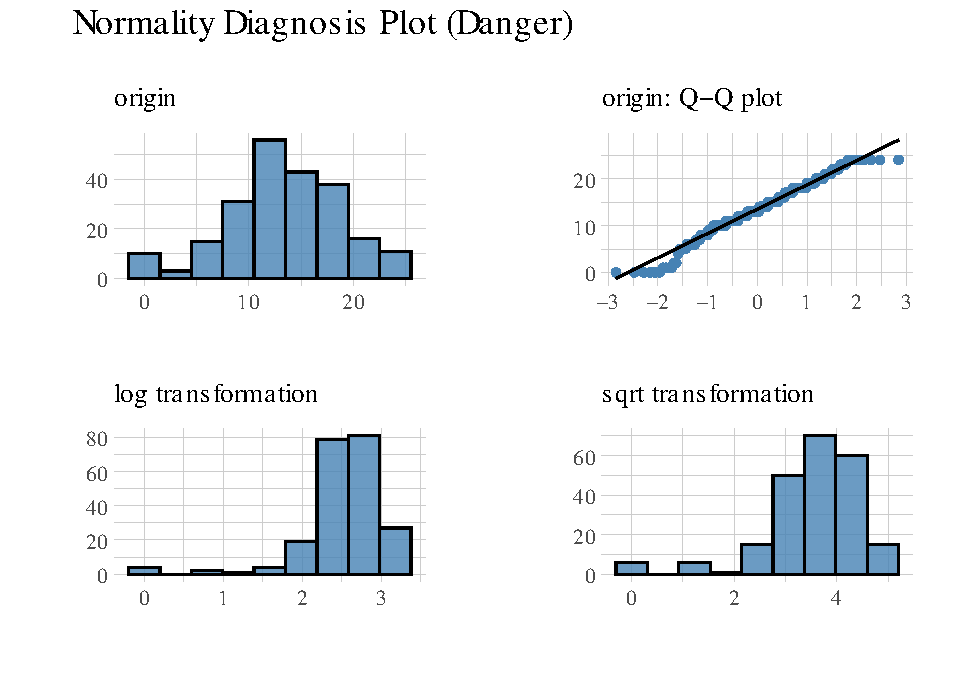
\includegraphics{bookdown-docentes_files/figure-latex/unnamed-chunk-5-1.pdf}

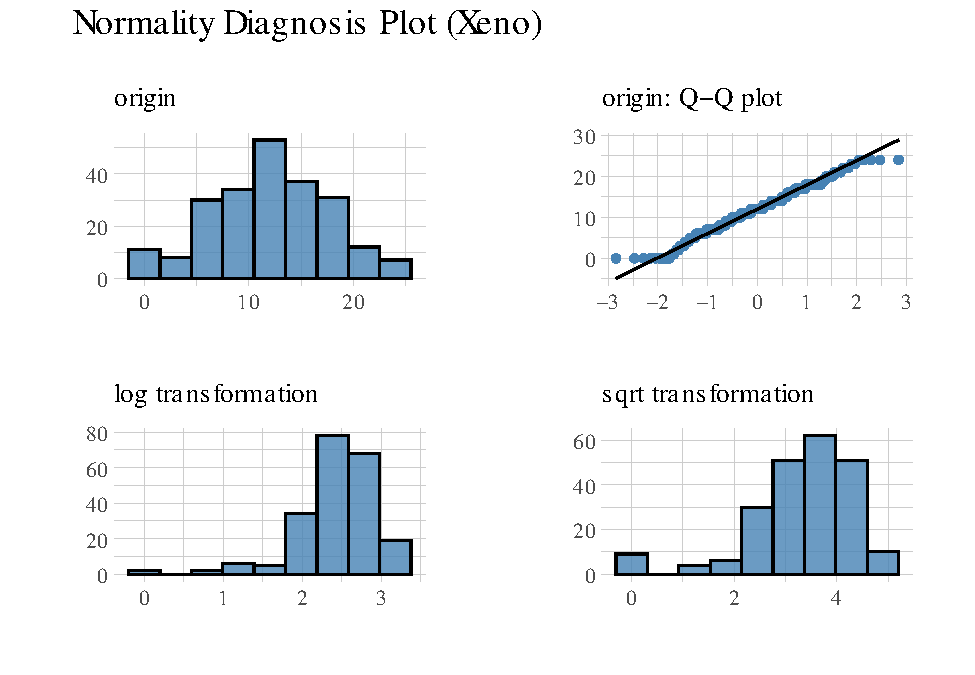
\includegraphics{bookdown-docentes_files/figure-latex/unnamed-chunk-6-1.pdf}

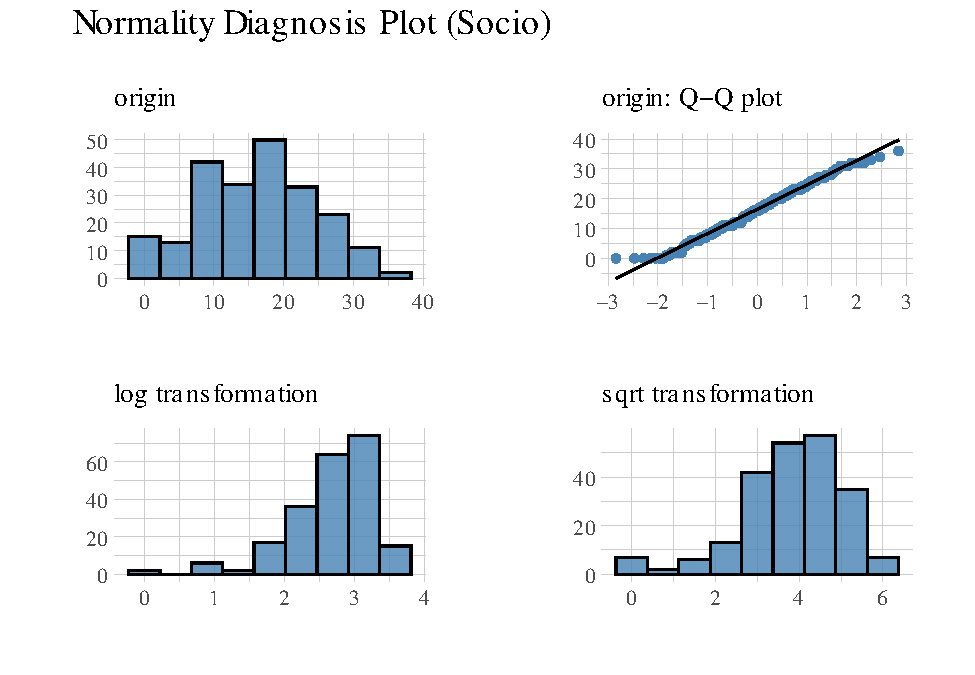
\includegraphics{bookdown-docentes_files/figure-latex/unnamed-chunk-7-1.pdf}

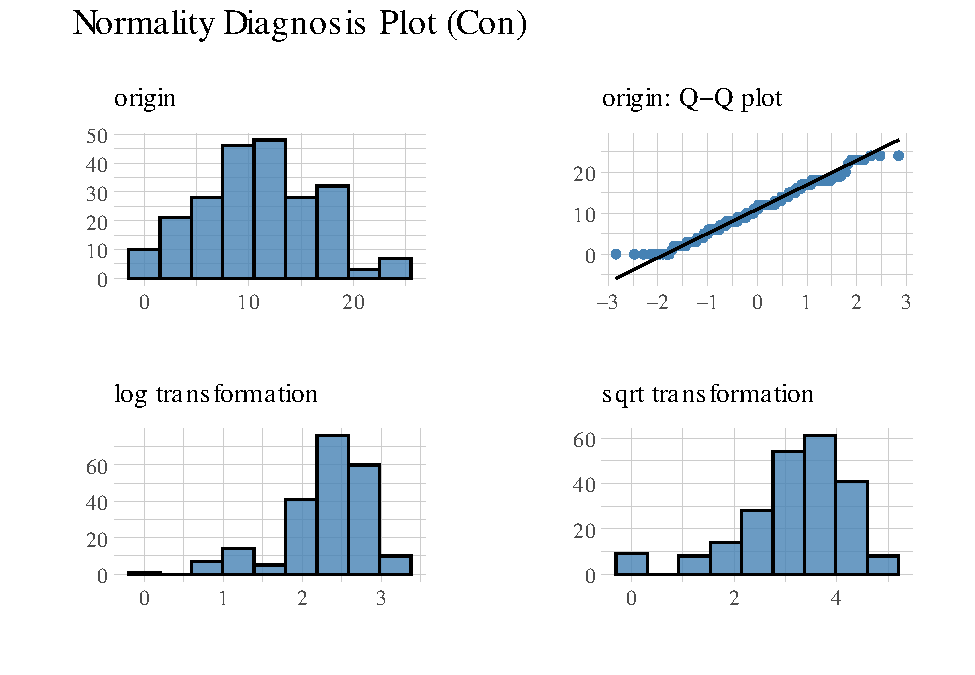
\includegraphics{bookdown-docentes_files/figure-latex/unnamed-chunk-8-1.pdf}

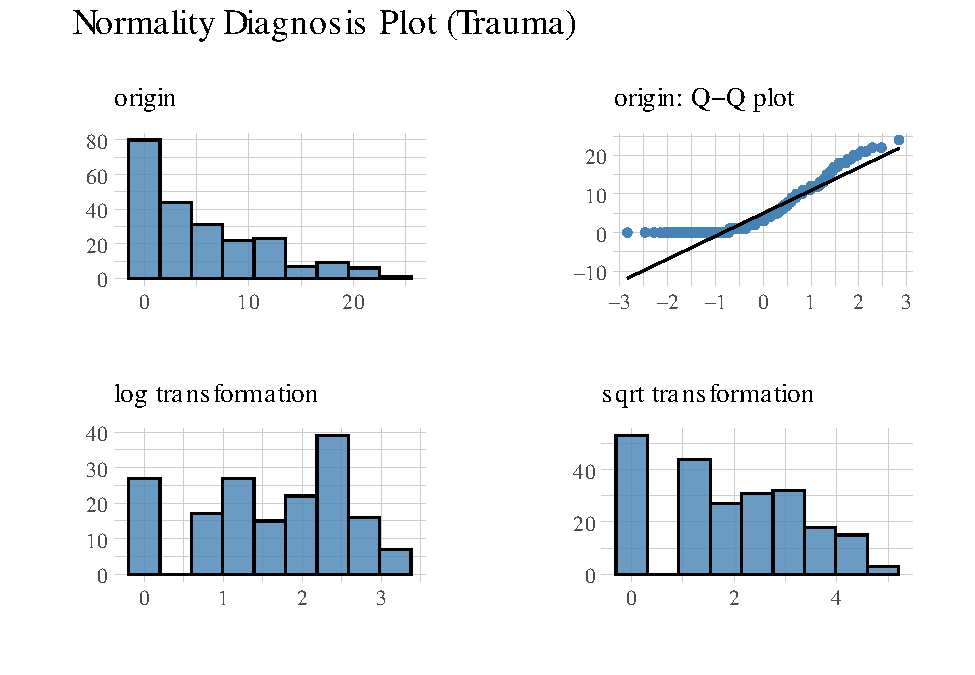
\includegraphics{bookdown-docentes_files/figure-latex/unnamed-chunk-9-1.pdf}

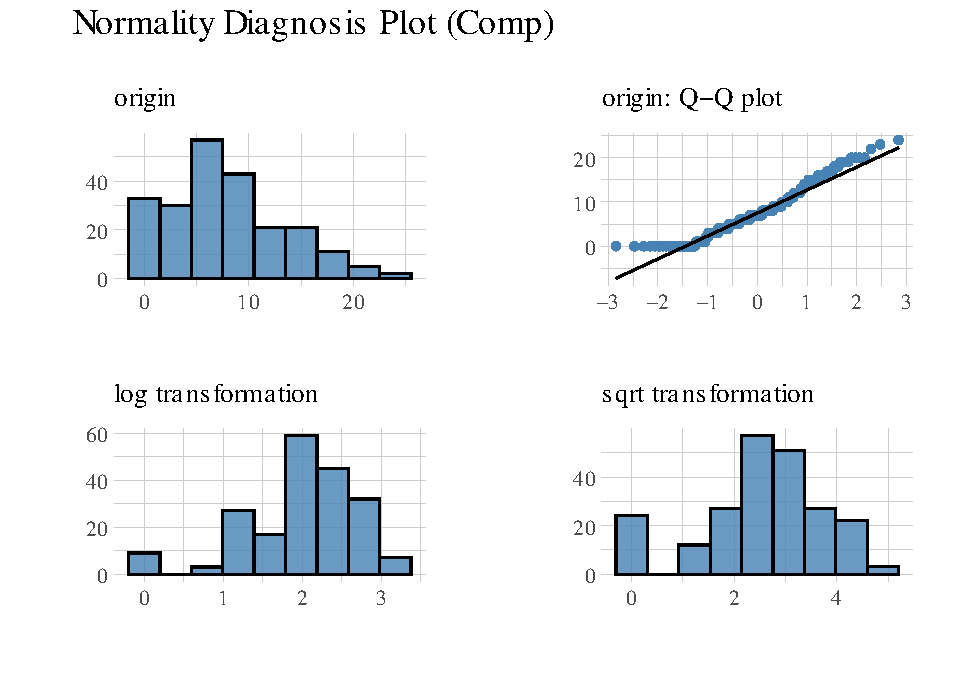
\includegraphics{bookdown-docentes_files/figure-latex/unnamed-chunk-10-1.pdf}

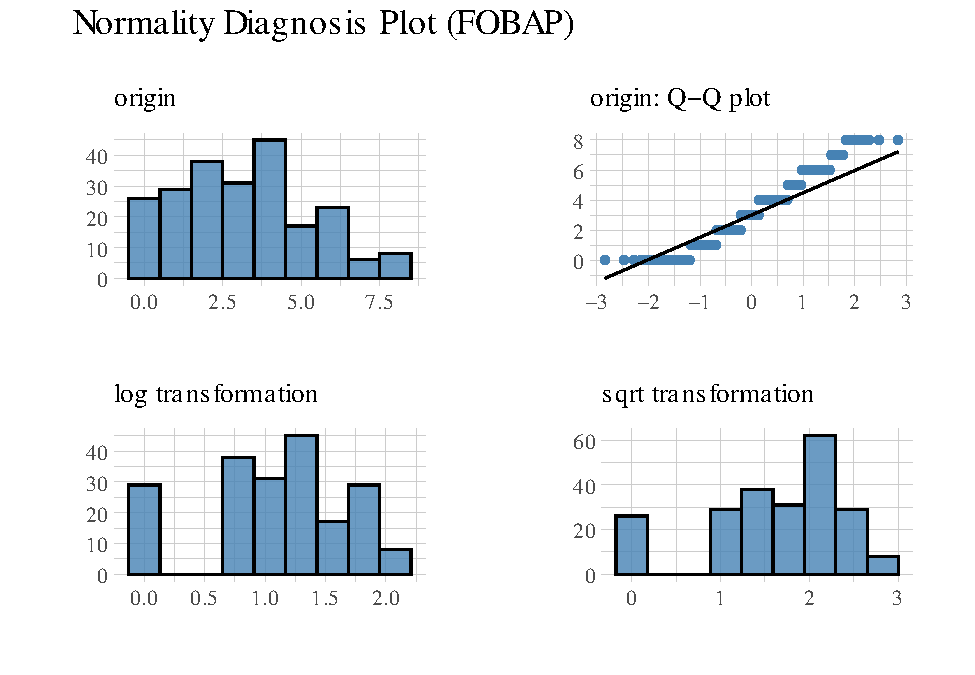
\includegraphics{bookdown-docentes_files/figure-latex/unnamed-chunk-11-1.pdf}

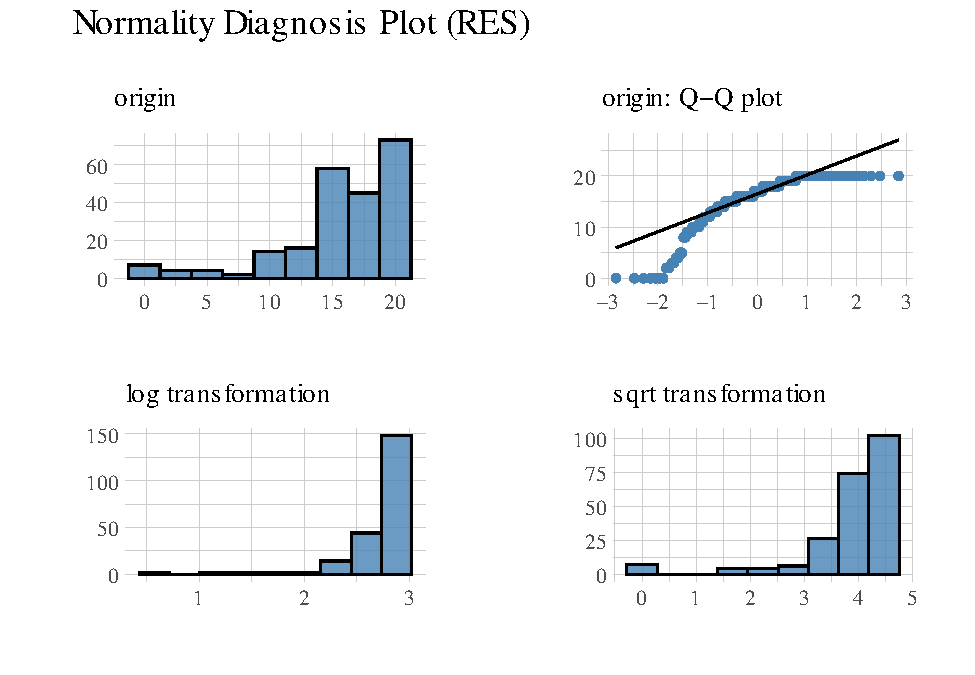
\includegraphics{bookdown-docentes_files/figure-latex/unnamed-chunk-12-1.pdf}

\hypertarget{anuxe1lisis-bivariado}{%
\section{Análisis Bivariado}\label{anuxe1lisis-bivariado}}

\begin{table}[H]
\centering
\begin{tabular}[t]{l|l|r}
\hline
var1 & var2 & coef\_corr\\
\hline
Xeno & Danger & 0.8315725\\
\hline
Socio & Danger & 0.6757264\\
\hline
Con & Danger & 0.6856952\\
\hline
Trauma & Danger & 0.5800335\\
\hline
Comp & Danger & 0.5397050\\
\hline
FOBAP & Danger & 0.6300303\\
\hline
RES & Danger & 0.2233475\\
\hline
Danger & Xeno & 0.8315725\\
\hline
Socio & Xeno & 0.7470481\\
\hline
Con & Xeno & 0.7390266\\
\hline
Trauma & Xeno & 0.5240995\\
\hline
Comp & Xeno & 0.4792495\\
\hline
FOBAP & Xeno & 0.5819781\\
\hline
RES & Xeno & 0.1164122\\
\hline
Danger & Socio & 0.6757264\\
\hline
Xeno & Socio & 0.7470481\\
\hline
Con & Socio & 0.7419982\\
\hline
Trauma & Socio & 0.4993905\\
\hline
Comp & Socio & 0.4833135\\
\hline
FOBAP & Socio & 0.4788010\\
\hline
RES & Socio & 0.1406821\\
\hline
Danger & Con & 0.6856952\\
\hline
Xeno & Con & 0.7390266\\
\hline
Socio & Con & 0.7419982\\
\hline
Trauma & Con & 0.4659353\\
\hline
Comp & Con & 0.5155762\\
\hline
FOBAP & Con & 0.5580933\\
\hline
RES & Con & 0.1757603\\
\hline
Danger & Trauma & 0.5800335\\
\hline
Xeno & Trauma & 0.5240995\\
\hline
Socio & Trauma & 0.4993905\\
\hline
Con & Trauma & 0.4659353\\
\hline
Comp & Trauma & 0.6139690\\
\hline
FOBAP & Trauma & 0.5580095\\
\hline
RES & Trauma & -0.0517958\\
\hline
Danger & Comp & 0.5397050\\
\hline
Xeno & Comp & 0.4792495\\
\hline
Socio & Comp & 0.4833135\\
\hline
Con & Comp & 0.5155762\\
\hline
Trauma & Comp & 0.6139690\\
\hline
FOBAP & Comp & 0.5247354\\
\hline
RES & Comp & 0.1239755\\
\hline
Danger & FOBAP & 0.6300303\\
\hline
Xeno & FOBAP & 0.5819781\\
\hline
Socio & FOBAP & 0.4788010\\
\hline
Con & FOBAP & 0.5580933\\
\hline
Trauma & FOBAP & 0.5580095\\
\hline
Comp & FOBAP & 0.5247354\\
\hline
RES & FOBAP & 0.0466312\\
\hline
Danger & RES & 0.2233475\\
\hline
Xeno & RES & 0.1164122\\
\hline
Socio & RES & 0.1406821\\
\hline
Con & RES & 0.1757603\\
\hline
Trauma & RES & -0.0517958\\
\hline
Comp & RES & 0.1239755\\
\hline
FOBAP & RES & 0.0466312\\
\hline
\end{tabular}
\end{table}

\hypertarget{matriz-de-correlaciuxf3n-variables-numuxe9ricas}{%
\subsection{Matriz de correlación, variables numéricas}\label{matriz-de-correlaciuxf3n-variables-numuxe9ricas}}

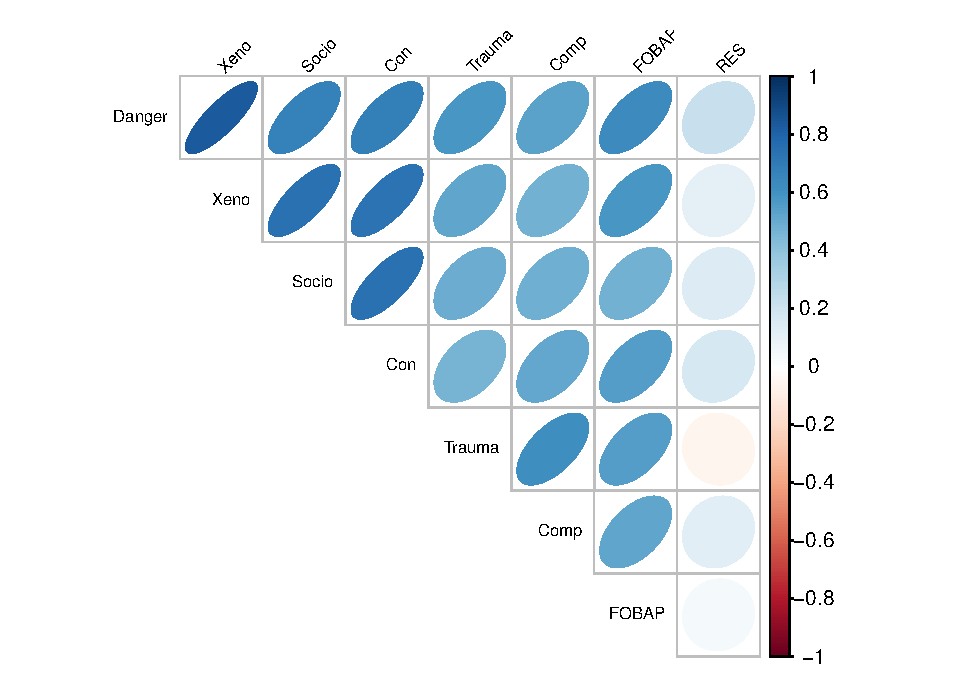
\includegraphics{bookdown-docentes_files/figure-latex/unnamed-chunk-14-1.pdf}

  \bibliography{book.bib,packages.bib}

\end{document}
